\section{Atari environments}
\label{envs}
\label{sec:envs}
% \todo[inline]{Here we describe interesting environments; this was quite nicely done in Chiappa's work as well as in Oh's work and this is the place where we want to discuss BankHeist}
In this section we describe \pong, \breakout\ and \freeway\ environments. These environments were introduced in the Arcade Learning Environment (ALE) \cite{ale} (see also \cite{ale2} for a current overview of challenges and successes of various learning methods in ALE). 

\paragraph{Dimensions of input and output.} The screen as given by the ALE emulator consists of an RGB image of the size $160\times 210$ pixels\todo[inline]{Is it rally true?}.  The action space consists of up to 18 actions. The reward in all games is an integer number.

\paragraph{\pong.} In \pong\ the player is expected to move the green paddle. The red paddle is operated by the original game AI. If the ball crosses the left end of the screen, then the green player scores a point. If the ball crosses the right end of the screen, then the red player scores a point. The total reward for the game is the difference between points scored by the green player and the red player. A full episode lasts until one of the agents scores 21 points. An environment for \pong\ was trained in \cite{recurrent}. Authors reported occasional disappearance of the ball and blurriness of paddles. In order to simplify learning of the environment we considered a modified environment with a ball of the size $10\times 10$ pixels. The change concerns only the observation and not rules of the game. 

\begin{figure}[H]
\makebox[\textwidth]{%
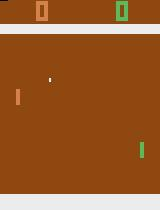
\includegraphics[width=0.24\textwidth]{figures/PongDeterministic-v4__0}%
\hfill    
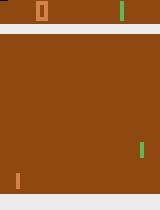
\includegraphics[width=0.24\textwidth]{figures/PongDeterministic-v4__3.jpg}%
\hfill
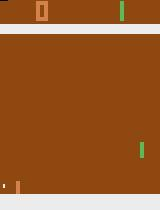
\includegraphics[width=0.24\textwidth]{figures/PongDeterministic-v4__9.jpg}%
\hfill    
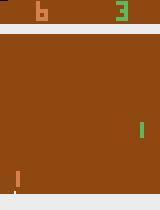
\includegraphics[width=0.24\textwidth]{figures/PongDeterministic-v4__31.jpg}%
}%
\caption{Four frames from the \pong\ environment. }
\label{fig:pong_original}
\end{figure}


\paragraph{\breakout.} In \breakout\ the player is expected to move the paddle located at the bottom of the screen. The paddle can be moved in the and right directions to the end of the screen. When the ball hits the wall of the bricks, points are scored depending on the color of the brick. The player has 5 lives and the beginning of the game. A life is lost whenever the ball crosses the bottom of the screen.  The environment makes appearance in \cite{recurrent} and is considered as a difficult environment to model \cite[page 18]{recurrent}. As in the case of \pong\ in the modified environment we allowed for a ball of the size $10\times 10$ pixels.

%\begin{comment}
\begin{figure}[H]
\makebox[\textwidth]{%
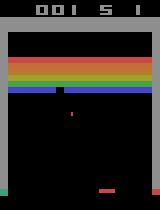
\includegraphics[width=0.24\textwidth]{figures/BreakoutDeterministic-v4__0}%
\hfill    
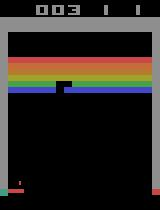
\includegraphics[width=0.24\textwidth]{figures/BreakoutDeterministic-v4__2.jpg}%
\hfill
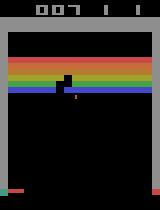
\includegraphics[width=0.24\textwidth]{figures/BreakoutDeterministic-v4__3.jpg}%
\hfill    
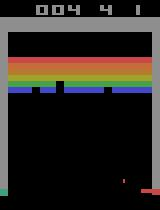
\includegraphics[width=0.24\textwidth]{figures/BreakoutDeterministic-v4__6.jpg}%
}%
\caption{Four frames from the original \breakout\ environment. }
\label{fig:breakout_original}
\end{figure}
%\end{comment}

\begin{comment}
\begin{figure}[H]
\makebox[\textwidth]{%
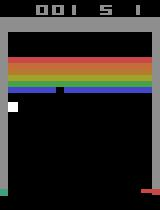
\includegraphics[width=0.24\textwidth]{figures_mod/BreakoutDeterministic-v4__0}%
\hfill    
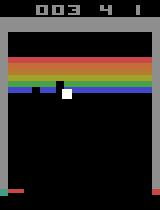
\includegraphics[width=0.24\textwidth]{figures_mod/BreakoutDeterministic-v4__1.jpg}%
\hfill
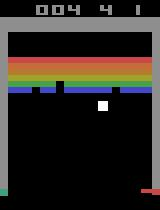
\includegraphics[width=0.24\textwidth]{figures_mod/BreakoutDeterministic-v4__2.jpg}%
\hfill    
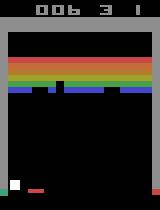
\includegraphics[width=0.24\textwidth]{figures_mod/BreakoutDeterministic-v4__4.jpg}%
}%
\caption{Four frames from the modified \breakout\ environment. }
\label{fig:breakout_mod}
\end{figure}
\end{comment}

\paragraph{\freeway.} In \freeway\ the player is expected to move the yellow chicken from the bottom of the screen to the top of the screen.  The chicken moves only vertically. A point is obtained in the game if the chicken reaches the top of the screen. There is no concept of life, but if the chicken is hit by a car, then it falls approximately 2 lanes down. The environment makes appearance in \cite{recurrent} and is considered as an easy environment to model \cite[page 18]{recurrent} frames. The problem though are the sparse rewards, since the only time a non-0 reward occurs is at the top of the screen.   % located at the bottom of the screen. The paddle can be moved in the and right directions to the end of the screen. When the ball hits the wall of the bricks, points are scored depending on the color of the brick. The player has 5 lives and the beginning of the game. A life is lost whenever the ball crosses the bottom of the screen.  The environment makes appearance in \cite{recurrent} and is considered as a difficult environment to model \cite[page 18]{recurrent}.  

%\begin{comment}
\begin{figure}[H]
\makebox[\textwidth]{%
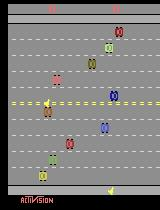
\includegraphics[width=0.24\textwidth]{figures/FreewayDeterministic-v4__0}%
\hfill    
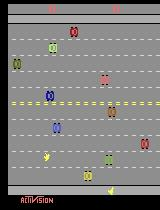
\includegraphics[width=0.24\textwidth]{figures/FreewayDeterministic-v4__4.jpg}%
\hfill
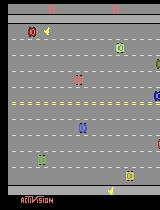
\includegraphics[width=0.24\textwidth]{figures/FreewayDeterministic-v4__6.jpg}%
\hfill    
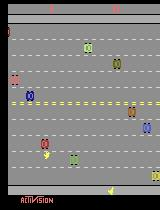
\includegraphics[width=0.24\textwidth]{figures/FreewayDeterministic-v4__8.jpg}%
}%
\caption{Four frames from the original \freeway\ environment. }
\label{fig:breakout_mode}
\end{figure}
% \end{comment}

\paragraph{\bankh.} \todo[inline]{Here Łukasz includes his take on \bankh}
